\documentclass{beamer}
\usepackage{ctex}
\usepackage{tikz,tikz-3dplot}
\usetheme{focus}
\tikzset{
    global scale/.style={scale=#1,every node/.append style={scale=#1}},
    CC1/.style ={circle,minimum width = 30pt, minimum height =30pt, draw},
    CC2/.style ={circle,minimum width = 30pt, minimum height =30pt, draw, fill=blue!20},
    RA1/.style ={rectangle,minimum width = 30pt, minimum height =20pt, draw},
    RA2/.style ={rectangle,minimum width = 1cm, minimum height = 1cm, draw},
    SU/.style ={very near start,sloped,above},
    NU/.style={near start,sloped,above}}

\begin{document}

\begin{frame}{8-1}
    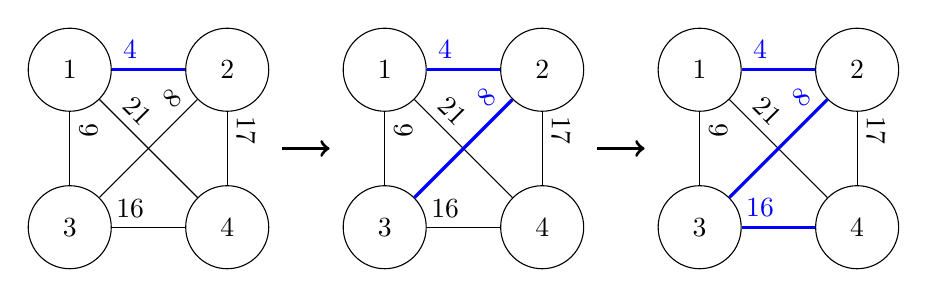
\begin{tikzpicture}
        \node[CC1] (3) at(0,0){3};
        \node[CC1] (4) at(2,0){4};
        \node[CC1] (7) at(4,0){3};
        \node[CC1] (8) at(6,0){4};
        \node[CC1] (11) at(8,0){3};
        \node[CC1] (12) at(10,0){4};
        \node[CC1] (1) at(0,2){1};
        \node[CC1] (2) at(2,2){2};
        \node[CC1] (5) at(4,2){1};
        \node[CC1] (6) at(6,2){2};
        \node[CC1] (9) at(8,2){1};
        \node[CC1] (10) at(10,2){2};
        \draw [very thick,blue](1) --(2) node[NU]{4};
        \draw (1) --(3) node[NU]{9};
        \draw (1) --(4) node[NU]{21};
        \draw (2) --(3) node[SU]{8};
        \draw (2) --(4) node[NU]{17};
        \draw (3) --(4) node[NU]{16};
        \draw [very thick,blue](5) --(6) node[NU]{4};
        \draw (5) --(7) node[NU]{9};
        \draw (5) --(8) node[NU]{21};
        \draw [very thick,blue](6) --(7) node[SU]{8};
        \draw (6) --(8) node[NU]{17};
        \draw (7) --(8) node[NU]{16};
        \draw [very thick,blue](9) --(10) node[NU]{4};
        \draw (9) --(11) node[NU]{9};
        \draw (9) --(12) node[NU]{21};
        \draw [very thick,blue](10) --(11) node[SU]{8};
        \draw (10) --(12) node[NU]{17};
        \draw [very thick,blue](11) --(12) node[NU]{16};
        \draw[->,very thick] (2.7,1)--(3.3,1);
        \draw[->,very thick] (6.7,1)--(7.3,1);
    \end{tikzpicture}
\end{frame}
\begin{frame}{8-2}
    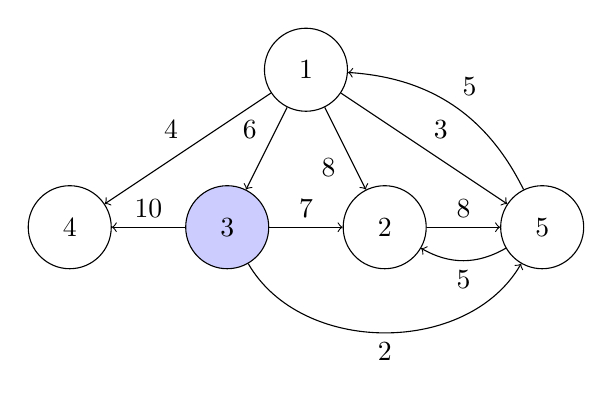
\begin{tikzpicture}
        \node[CC1] (5) at(6,0){5};
        \node[CC1] (4) at(0,0){4};
        \node[CC1,fill=blue!20] (3) at(2,0){3}
            edge[->]node[auto,swap] {10}(4)
            edge[->,bend right=60]node[auto,swap] {2}(5);
        \node[CC1] (2) at(4,0){2}
            edge[<-]node[auto,swap] {7}(3)
            edge[->]node[auto] {8}(5)
            edge[<-,bend right]node[auto,swap] {5}(5);
        \node[CC1] (1) at(3,2){1}
            edge[->]node[auto,swap] {8}(2)
            edge[->]node[auto,swap] {6}(3)
            edge[->]node[auto,swap] {4} (4)
            edge[->]node[auto] {3}(5)
            edge[<-,bend left]node[auto] {5}(5);
    \end{tikzpicture}
\end{frame}
\begin{frame}{8-5}
    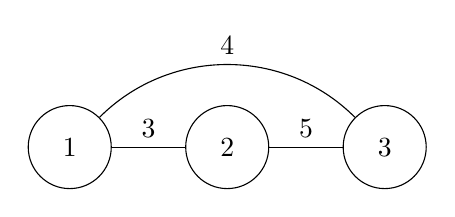
\begin{tikzpicture}
        \node[CC1] (1) at(0,0){1};
        \node[CC1] (2) at(2,0){2}
            edge node[auto,swap]{3}(1);
        \node[CC1] (3) at(4,0){3}
            edge node[auto,swap]{5}(2)
            edge[bend right=45]node[auto,swap]{4}(1);
    \end{tikzpicture}
\end{frame}
\begin{frame}{8-6}
    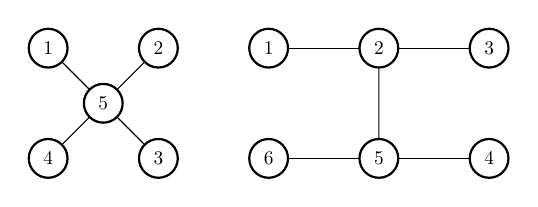
\begin{tikzpicture}
        [every node/.style={circle,minimum width=20pt,minimum height=20pt,thick,draw},
        edge/.style={thick,draw},global scale=0.7]
    \node(1) at(0,2){1};
    \node(2) at(2,2){2};
    \node(3) at(2,0){3};
    \node(4) at(0,0){4};
    \node(5) at(1,1){5}
        edge (1) edge (2) edge (3) edge (4);
    \node(6) at(4,2){1};
    \node(8) at(8,2){3};
    \node(7) at(6,2){2}
        edge (6) edge (8);
    \node(9) at(4,0){6};
    \node(11) at(8,0){4};
    \node(10) at(6,0){5}
        edge (7) edge (11) edge (9);
    \end{tikzpicture}
\end{frame}
\end{document}
